\documentclass[11pt,a4paper]{article}
\usepackage[margin=2.4cm]{geometry}
\usepackage{amsmath,amssymb,amsthm,bm,mathtools}
\usepackage{booktabs}
\usepackage{tikz}
\usetikzlibrary{decorations.pathmorphing,arrows.meta,patterns}
\usepackage[most]{tcolorbox}
\usepackage[colorlinks=true,linkcolor=blue!50!black,citecolor=blue!50!black,urlcolor=blue!50!black]{hyperref}
\usepackage{enumitem}
\emergencystretch=1.5em

\newcommand{\kT}{k_{\mathrm B}T}
\newcommand{\dd}{\mathrm{d}}
\newcommand{\avg}[1]{\left\langle #1\right\rangle}
\newcommand{\lam}{\bm{\lambda}}
\newcommand{\Wd}{W_{\rm diss}}
\newcommand{\dFJ}{\widehat{\Delta F}_J}
\newtcolorbox{note}[1][]{colback=blue!3,colframe=blue!40!black,fonttitle=\bfseries,title=#1}
\newtcolorbox{result}[1][]{colback=green!3,colframe=green!35!black,fonttitle=\bfseries,title=#1}

\title{Jarzynski equality for a pulled polymer in 2D\\[0.3em]
\large Theory companion: model, fluctuation theorems, estimators and numerical scheme}
\author{}
\date{9 October 2026 (first version 6 October 2026)}

\begin{document}
\maketitle

\begin{abstract}
This document gives the theory behind the simulations of the companion report
(\texttt{report.pdf}). It contains the model of an anchored 2D bead--spring chain pulled by a
moving harmonic trap in a Langevin bath. It derives the Jarzynski equality in three settings
(Hamiltonian, discrete-time Markov, continuous-time Langevin) and explains what the equality says
about the free energy. It derives the Crooks fluctuation theorem, and every estimator of $\Delta F$
used in the report: one-sided Jarzynski with its bias and variance, cumulant expansions, effective
sample size, reverse Jarzynski, and Bennett's acceptance ratio. It also describes the exact
free-energy references and the numerical scheme. The first version of this document was
written before any code. This version incorporates the design decisions taken and two corrections
found while running the simulations (Sec.~\ref{sec:decisions}).
\end{abstract}

\tableofcontents
\newpage

%=====================================================================
\section{Comments on the original brief}
\label{sec:corrections}

\begin{note}[Three points where the brief needed adjusting]
\begin{enumerate}[leftmargin=*]
\item \textbf{Random forces alone are not enough.} A bath has to do two things: kick the beads
(noise) \emph{and} slow them down (friction). With kicks only, every kick adds energy on
average, so $\avg{v^2}$ grows linearly in time and the chain heats up without bound.
Noise and friction come from the same molecular collisions, and their strengths are tied by
the fluctuation--dissipation relation $\sigma^2 = 2\gamma m\kT$ (Sec.~\ref{sec:bath}).
\item \textbf{What fluctuates is the work, not the free energy.} $\Delta F=F(\lam_1)-F(\lam_0)$
is a property of two \emph{equilibrium} states, so it is one number. The \emph{work} $W$ done by
the puller differs on every repetition; its distribution $P(W)$ is what changes with $T$, $N$
and speed. Jarzynski extracts the single number $\Delta F$ from the distribution of irreversible works.
\item \textbf{How the chain is pulled.} Instead of moving the last bead along a prescribed path
(a constraint), the last bead is held in a harmonic trap whose centre $\lam(t)$ moves, as in
optical-tweezer and AFM experiments. The work is then an explicit formula (Eq.~\ref{eq:work}).
\end{enumerate}
\end{note}

%=====================================================================
\section{Physical model}
\label{sec:model}

\begin{figure}[h]
\centering
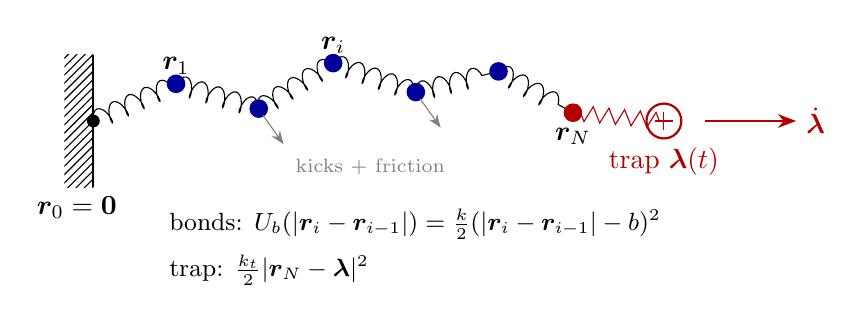
\begin{tikzpicture}[scale=1.05]
  \fill[pattern=north east lines] (-0.35,-0.8) rectangle (0,0.8);
  \draw[thick] (0,-0.8)--(0,0.8);
  \coordinate (r0) at (0,0);
  \coordinate (r1) at (1.0,0.45);
  \coordinate (r2) at (2.0,0.15);
  \coordinate (r3) at (2.9,0.7);
  \coordinate (r4) at (3.9,0.35);
  \coordinate (r5) at (4.9,0.6);
  \coordinate (r6) at (5.8,0.1);
  \foreach \a/\b in {r0/r1,r1/r2,r2/r3,r3/r4,r4/r5,r5/r6}
    \draw[decorate,decoration={coil,aspect=0.4,segment length=2.2mm,amplitude=1.2mm}] (\a)--(\b);
  \fill[black] (r0) circle (2.2pt);
  \foreach \p in {r1,r2,r3,r4,r5} \fill[blue!60!black] (\p) circle (3.2pt);
  \fill[red!70!black] (r6) circle (3.2pt);
  \node at (-0.2,-1.05) {$\bm r_0=\bm 0$};
  \node[above] at (r1) {$\bm r_1$};
  \node[above] at (r3) {$\bm r_i$};
  \node[below=2pt] at (r6) {$\bm r_N$};
  \coordinate (lam) at (6.9,0);
  \draw[red!70!black,decorate,decoration={zigzag,segment length=2mm,amplitude=1mm}] (r6)--(lam);
  \draw[red!70!black,thick] (lam) circle (6pt);
  \draw[red!70!black] (lam) +(-3pt,0)--+(3pt,0) +(0,-3pt)--+(0,3pt);
  \node[below=6pt,red!70!black] at (lam) {trap $\lam(t)$};
  \draw[-{Stealth},thick,red!70!black] (7.4,0)--(8.5,0) node[right] {$\dot{\lam}$};
  \node[anchor=west] at (0.8,-1.25) {\small bonds: $U_b(|\bm r_i-\bm r_{i-1}|)=\tfrac{k}{2}(|\bm r_i-\bm r_{i-1}|-b)^2$};
  \node[anchor=west] at (0.8,-1.8) {\small trap: $\tfrac{k_t}{2}|\bm r_N-\lam|^2$};
  \foreach \p in {r2,r4} \draw[-{Stealth},gray] (\p)++(0.05,-0.08) -- ++(0.25,-0.35);
  \node[gray] at (3.35,-0.55) {\scriptsize kicks + friction};
\end{tikzpicture}
\caption{The system. Bead $0$ is fixed at the origin; beads $1\dots N$ move in the plane and
exchange energy with the bath; bead $N$ is held by a harmonic trap whose centre moves from
$\lam_0$ to $\lam_1$ in a time $\tau$.}
\label{fig:schematic}
\end{figure}

The state is $\bm x=(\bm r_1,\dots,\bm r_N;\bm p_1,\dots,\bm p_N)\in\mathbb R^{4N}$, with
$\bm r_0\equiv\bm 0$. The Hamiltonian depends on the control parameter $\lam\in\mathbb R^2$:
\begin{equation}
H(\bm x;\lam) = \sum_{i=1}^N \frac{|\bm p_i|^2}{2m}
 + \sum_{i=1}^N U_b\big(|\bm r_i-\bm r_{i-1}|\big)
 + \frac{k_t}{2}\,|\bm r_N-\lam|^2,
\qquad U_b(r)=\frac{k}{2}(r-b)^2 .
\label{eq:H}
\end{equation}
$N$ is the number of mobile beads, which equals the number of bonds.

\paragraph{One model, two limits.}
\begin{itemize}[leftmargin=*]
\item $b=0$, \textbf{Gaussian (Rouse) chain}: all forces are linear, so the free energy, the dynamics
and the full work distribution are known exactly (Sec.~\ref{sec:exactA}). The elasticity is
\emph{energetic}. Role: validation.
\item $b=1$, stiff bonds ($kb^2\gg\kT$), \textbf{nearly freely-jointed chain}: bond lengths barely
change, so pulling works against \emph{entropy} (rubber elasticity, restoring force $\propto T$).
Role: the physics model.
\end{itemize}
\paragraph{Simplifications.} The chain is a phantom chain (no excluded volume, which is what makes
the exact reference of Sec.~\ref{sec:exactB} possible), it has no bending stiffness, and the bath
is free-draining (no hydrodynamic interactions).

\paragraph{Protocol.} $\lam(t)=\big(x_0+(x_1-x_0)t/\tau,\,0\big)$ with $x_0=0.2L$, $x_1=0.7L$, where
$L=Nb$ is the contour length ($L=0.3N$ for $b=0$). The chain starts in equilibrium at $\lam_0$. The
\emph{reverse} protocol, used for Crooks, runs $x_1\to x_0$ in the same time, starting in equilibrium at $\lam_1$.

\paragraph{Units and parameters.} $m=b=\varepsilon=1$; $k=100$, $k_t=10$, $\gamma=1$
($\zeta=m\gamma$), $\Delta t=0.01$, $M=10^5$ pulls per parameter set; $\kT\in\{0.25,0.5,1,2\}$,
$N\in\{5,10,20,40\}$.

%=====================================================================
\section{The heat bath: Langevin dynamics}
\label{sec:bath}

Each mobile bead obeys
\begin{equation}
\dd\bm r_i=\frac{\bm p_i}{m}\,\dd t,\qquad
\dd\bm p_i = -\nabla_{\bm r_i}H(\bm x;\lam(t))\,\dd t - \gamma\,\bm p_i\,\dd t
 + \sqrt{2\gamma m\kT}\;\dd\bm B_i(t),
\label{eq:langevin}
\end{equation}
with independent 2D Wiener processes $\bm B_i$.

\paragraph{Why the noise strength must be $2\gamma m\kT$.} For one free bead in 1D,
$\dd p=-\gamma p\,\dd t+\sigma\,\dd B$. It\^o's lemma gives $\dd(p^2)=2p\,\dd p+\sigma^2\dd t$, hence
$\tfrac{\dd}{\dd t}\avg{p^2}=-2\gamma\avg{p^2}+\sigma^2$ and $\avg{p^2}\to\sigma^2/2\gamma$.
Equipartition ($\avg{p^2}=m\kT$) requires $\sigma^2=2\gamma m\kT$. With $\gamma=0$ (``random
forces only'') $\avg{p^2}=\sigma^2t$ grows without bound.

\subsection{Stationary distribution: why the bath produces the canonical ensemble}
\label{sec:stationary}

\paragraph{Why we need this.} Three things in this project rest on one fact: at a frozen trap
position $\lam$, the Langevin dynamics \eqref{eq:langevin} relaxes to the canonical distribution
\begin{equation}
\rho_{\rm eq}(\bm x;\lam)=\frac{e^{-\beta H(\bm x;\lam)}}{Z(\lam)},\qquad
Z(\lam)=\int e^{-\beta H(\bm x;\lam)}\,\dd\bm x,\qquad\beta=\frac1{\kT}.
\label{eq:rhoeq}
\end{equation}
(i) The free energy $F=-\kT\ln Z$ is defined with respect to it. (ii) Every pull must start from it.
(iii) The proof of the Jarzynski equality (Sec.~\ref{sec:jarzynski}) uses \emph{only} the property
that the dynamics at frozen $\lam$ leaves $\rho_{\rm eq}$ unchanged. This subsection shows where that property comes from.

\paragraph{Two descriptions of the same dynamics.} Equation \eqref{eq:langevin} describes one random
trajectory. Averaging over the noise gives the evolution of the probability density $\rho(\bm x,t)$
of the state. The bridge between the two is the \emph{generator} $\mathcal L$, defined by how the
average of any observable $f(\bm x)$ changes:
\begin{equation}
\frac{\dd}{\dd t}\avg{f(\bm x_t)}=\avg{(\mathcal Lf)(\bm x_t)} .
\end{equation}
It follows from It\^o's lemma: $\dd f=\nabla_{\bm r}f\cdot\dd\bm r+\nabla_{\bm p}f\cdot\dd\bm p
+\tfrac12(2\gamma m\kT)\Delta_{\bm p}f\,\dd t$. The last term comes from $(\dd B)^2=\dd t$; the noise term
itself averages to zero. Inserting \eqref{eq:langevin},
\begin{equation}
\mathcal Lf=\underbrace{\frac{\bm p}{m}\cdot\nabla_{\bm r}f-\nabla_{\bm r}H\cdot\nabla_{\bm p}f}_{\mathcal L^{\rm ham}f\ \text{(Newton)}}
\;+\;\gamma\underbrace{\big(-\bm p\cdot\nabla_{\bm p}f+m\kT\,\Delta_{\bm p}f\big)}_{\mathcal L^{\rm OU}f\ \text{(friction + noise)}} .
\end{equation}
Since $\avg{f(\bm x_t)}=\int f\rho_t\,\dd\bm x$, an integration by parts moves $\mathcal L$ from $f$ onto
$\rho$. The density obeys the Fokker--Planck (here: Kramers) equation $\partial_t\rho=\mathcal L^\dagger\rho$, with the
adjoint operator
\begin{equation}
\mathcal L^\dagger\rho=\underbrace{-\frac{\bm p}{m}\cdot\nabla_{\bm r}\rho+\nabla_{\bm r}H\cdot\nabla_{\bm p}\rho}_{\mathcal L^{\rm ham\dagger}\rho}
\;+\;\gamma\,\underbrace{\nabla_{\bm p}\cdot\big(\bm p\,\rho+m\kT\,\nabla_{\bm p}\rho\big)}_{\mathcal L^{\rm OU\dagger}\rho}.
\end{equation}
A density is \emph{stationary} if $\mathcal L^\dagger\rho=0$. We check the two parts separately for $\rho=e^{-\beta H}/Z$.

\paragraph{Hamiltonian part: any function of the energy is stationary.} Take any $\rho=\phi(H)$.
Then $\nabla_{\bm r}\rho=\phi'\,\nabla_{\bm r}H$ and $\nabla_{\bm p}\rho=\phi'\,\bm p/m$, so
\[
\mathcal L^{\rm ham\dagger}\rho=\phi'\Big(-\frac{\bm p}{m}\cdot\nabla_{\bm r}H+\nabla_{\bm r}H\cdot\frac{\bm p}{m}\Big)=0 .
\]
This is energy conservation (Liouville). Newton's equations alone do not choose a temperature:
$e^{-\beta H}$ is stationary for \emph{every} $\beta$, and so is any other function of $H$.

\paragraph{Friction and noise select the temperature.} The OU part is the divergence of a probability
current in momentum space, $\bm J_{\bm p}=-(\bm p\rho+m\kT\nabla_{\bm p}\rho)$. For $\rho\propto e^{-\beta H}$,
$\nabla_{\bm p}\rho=-\beta(\bm p/m)\rho$, so $m\kT\,\nabla_{\bm p}\rho=-\bm p\rho$ and the current vanishes
\emph{identically}: friction pushes probability towards $\bm p=0$, and the noise spreads it out
again at exactly the same rate. Had we used a noise strength $\sigma^2$ instead of $2\gamma m\kT$,
the current would be $\bm p\rho\,(\sigma^2/2\gamma m\kT-1)\neq0$ unless $\sigma^2=2\gamma m\kT$. Only one
temperature is stationary, the one fixed by the fluctuation--dissipation relation.

\paragraph{Uniqueness and relaxation.} Because the noise acts on the momenta and the forces couple
momenta to positions, the dynamics explores the whole phase space. $\rho_{\rm eq}$ is then the
\emph{unique} stationary density, and any initial density relaxes to it (hypocoercivity). This is
what ``the chain is thermalised by the bath'' means mathematically. When $\lam$ moves, $\rho_{\rm eq}(\lam(t))$
is no longer stationary and the chain lags behind it; the work that this lag costs is the dissipated work.

\subsection{Slowest relaxation time $\tau_1$}
\label{sec:tau1}

\paragraph{What it is for.} Whether a pull is ``fast'' or ``slow'' only makes sense relative to how
quickly the chain can re-equilibrate. We measure every pulling time in units of $\tau_1$, the
relaxation time of the slowest collective motion of the chain. If $\tau\gg\tau_1$ the chain follows the
trap almost in equilibrium (little dissipation). If $\tau\lesssim\tau_1$ the chain lags behind and
dissipates a lot. $\tau_1$ sets the scale; it does not enter any of the measured quantities.

\paragraph{Step 1: overdamped description at the chain scale.} Momenta relax on the time $1/\gamma=1$,
much shorter than the collective times we are after (tens to hundreds of time units). On those scales
inertia is negligible, and each bead obeys the overdamped (Brownian) equation
$\zeta\,\dot{\bm r}_i=\bm F_i+\text{noise}$, with friction coefficient $\zeta=m\gamma$.

\paragraph{Step 2: replace the chain by linear springs.} For $b=0$ the bonds are already linear springs
of stiffness $\kappa=k$. For $b=1$ the bonds hardly stretch, but a \emph{segment} of the chain behaves as
a spring of entropic origin. By the central limit theorem, the end-to-end vector of $n$ freely jointed
bonds is Gaussian, with each Cartesian component having variance $n\avg{u^2}/2$ in 2D. Its free
energy is therefore $F(\bm R)=-\kT\ln P(\bm R)=\kT|\bm R|^2/(n\avg{u^2})+$const: a harmonic spring of stiffness
$\kappa/n$ with
\begin{equation}
\kappa=\frac{2\kT}{\avg{u^2}}\qquad\text{per bond (2D entropic spring)}.
\end{equation}
This is the Rouse model: each bond is replaced by an entropic spring. For $\kT=1$, $\kappa\approx1.94$,
about $50\times$ softer than the bond itself ($k=100$).

\paragraph{Step 3: normal modes.} With linear springs the overdamped equations read
$\zeta\,\dot{\bm r}=-K\bm r+\text{(trap force at fixed }\lam)+\text{noise}$, separately for $x$ and $y$.
$K$ is the $N\times N$ stiffness matrix: $K_{ii}=2\kappa$ for $i<N$, $K_{NN}=\kappa+k_t$ (the last bead
has one bond and the trap), $K_{i,i\pm1}=-\kappa$. The anchored bead $0$ is fixed and does not appear.
Writing the deviation from the mean shape in the eigenvectors of $K$, each mode $p$ relaxes
independently as $e^{-\lambda_pt/\zeta}$. The slowest one defines
\begin{equation}
\tau_1=\frac{\zeta}{\lambda_{\min}(K)} ,
\end{equation}
which is what the code computes (\texttt{params.tau1}).

\paragraph{Step 4: closed-form estimate.} Since $k_t=10\gg\kappa\approx2$, the trap holds bead $N$ almost fixed,
so the chain is effectively clamped at both ends. The modes of a discrete string fixed at both ends are
$\sin(p\pi i/N)$, with eigenvalues $\lambda_p=4\kappa\sin^2(p\pi/2N)\simeq\kappa(p\pi/N)^2$. The slowest is
the half-wave $p=1$:
\begin{equation}
\tau_1\simeq\frac{\zeta}{\kappa}\Big(\frac{N}{\pi}\Big)^2=\frac{\zeta N^2\avg{u^2}}{2\pi^2\kT}
\qquad(b=1).
\label{eq:rouse}
\end{equation}
For $N=10$ this gives $5.22$, against the exact eigenvalue $5.46$ (the trap is not infinitely stiff).
For $N=40$ it gives $83.5$, against $84.3$.

\paragraph{What the formula says.} $\tau_1\propto N^2$ (Rouse scaling: a disturbance diffuses along the chain
with a diffusion constant $\kappa/\zeta$ per bead$^2$) and $\tau_1\propto\zeta$. For the entropic
chain $\tau_1\propto1/T$, because the entropic spring is stiffer at high temperature; for the Gaussian
chain ($\kappa=k$) $\tau_1$ does not depend on $T$. Values: $\tau_1=1.45,5.46,21.3,84.3$ for
$N=5,10,20,40$ at $\kT=1$; $20.8$, $10.6$, $5.46$, $2.91$ for $\kT=0.25,0.5,1,2$ at $N=10$; $0.26$ for the
$b=0$ chain with $N=10$.

\emph{Correction to the first version:} it assumed a \emph{free} far end, whose slowest mode is the
quarter wave $\sin(\pi i/2N)$. That overestimates $\tau_1$ by a factor $4$.

%=====================================================================
\section{Equilibrium free energy}
\label{sec:F}

\paragraph{Definition.} With the canonical distribution \eqref{eq:rhoeq}, the free energy at fixed
$\lam$ is $F(\lam)=-\kT\ln Z(\lam)$, and
\begin{equation}
\Delta F=F(\lam_1)-F(\lam_0)=-\kT\ln\frac{Z(\lam_1)}{Z(\lam_0)} .
\label{eq:dFdef}
\end{equation}
Only \emph{ratios} of partition functions are physical here, so constant factors in $Z$ (the
momentum integral, normalisation of $\dd\bm x$) cancel. The kinetic energy does not depend on
$\lam$, so $\Delta F$ is a purely configurational quantity.

\paragraph{$\Delta F$ is the reversible work.} Differentiate $F$ with respect to $\lam$:
\begin{equation}
\frac{\partial F}{\partial\lam}=-\kT\,\frac{1}{Z}\frac{\partial Z}{\partial\lam}
=-\kT\,\frac1Z\int\Big(-\beta\frac{\partial H}{\partial\lam}\Big)e^{-\beta H}\dd\bm x
=\Big\langle\frac{\partial H}{\partial\lam}\Big\rangle_{\lam}.
\label{eq:meanforce}
\end{equation}
The derivative of the free energy is the equilibrium average of the generalised force. For the trap
this is $\partial_{\lam}H=-k_t(\bm r_N-\lam)$, i.e.\ minus the mean force the trap exerts on the
bead. If the trap is moved infinitely slowly, the chain stays in equilibrium at every $\lam$, so
the work is
$W_{\rm rev}=\int\avg{\partial_{\lam}H}_{\lam}\cdot\dd\lam=\int\partial_{\lam}F\cdot\dd\lam=\Delta F$.
This is also the basis of \emph{thermodynamic integration}: measure the mean force at a grid of
fixed $\lam$ and integrate. It is used as a check in the code.

\paragraph{Energy and entropy.} $\Delta F=\Delta U-T\Delta S$ with $\Delta S=-\partial\Delta F/\partial T$.
For the stiff-bond chain $\Delta F\approx T\,\phi(\lam_0,\lam_1)$ (Sec.~\ref{sec:exactB}), so
$\Delta U\approx0$ and $\Delta F\approx-T\Delta S$: the work goes into lowering the entropy of the
chain, and the same amount is released to the bath as heat. For the Gaussian chain $\Delta F$ is
independent of $T$ and is entirely stored as spring energy.

%=====================================================================
\section{Work, heat and the Jarzynski equality}
\label{sec:jarzynski}

\subsection{Work and heat along one trajectory}
Following Sekimoto, the change of energy along a trajectory splits into a part due to the control and
a part exchanged with the bath:
\begin{equation}
\dd H=\underbrace{\frac{\partial H}{\partial\lam}\cdot\dd\lam}_{\dd W}\;+\;
\underbrace{\nabla_{\bm x}H\circ\dd\bm x}_{\dd Q},
\qquad
W=\int_0^\tau\frac{\partial H}{\partial\lam}\cdot\dot\lam\,\dd t=-k_t\int_0^\tau(\bm r_N-\lam)\cdot\dot\lam\,\dd t .
\label{eq:work}
\end{equation}
$W$ is the work done by the puller and $Q=\Delta H-W$ the heat received from the bath.

\begin{note}[Jarzynski equality (1997)]
If (i) the system starts in equilibrium, $\bm x(0)\sim\rho_{\rm eq}(\cdot;\lam_0)$, and (ii) at every frozen
$\lam$ the dynamics leaves $\rho_{\rm eq}(\cdot;\lam)$ invariant, then for \emph{any} protocol
$\lam(t)$ and \emph{any} duration $\tau$,
\begin{equation}
\avg{e^{-\beta W}}=e^{-\beta\Delta F}.
\label{eq:JE}
\end{equation}
Neither detailed balance nor equilibrium at the end ($t=\tau$) is required.
\end{note}

\subsection{Proof 1: isolated Hamiltonian system (the original argument)}
Suppose the system is first equilibrated at $\lam_0$, then decoupled from the bath and driven by
Hamilton's equations. With no bath there is no heat, so
$W=H(\bm x_\tau;\lam_1)-H(\bm x_0;\lam_0)$, where $\bm x_\tau=\Phi(\bm x_0)$ is the deterministic
image of the initial point. Then
\begin{align}
\avg{e^{-\beta W}}
&=\int\dd\bm x_0\;\frac{e^{-\beta H(\bm x_0;\lam_0)}}{Z_0}\;
e^{-\beta[H(\Phi(\bm x_0);\lam_1)-H(\bm x_0;\lam_0)]}
=\frac1{Z_0}\int\dd\bm x_0\;e^{-\beta H(\Phi(\bm x_0);\lam_1)}\notag\\
&=\frac1{Z_0}\int\dd\bm x_\tau\;e^{-\beta H(\bm x_\tau;\lam_1)}=\frac{Z_1}{Z_0}=e^{-\beta\Delta F}.
\end{align}
The first step cancels the initial Boltzmann factor against the $e^{+\beta H(\bm x_0;\lam_0)}$ inside
$e^{-\beta W}$. The change of variables $\bm x_0\to\bm x_\tau$ has unit Jacobian by Liouville's theorem. The whole proof is
``the initial Boltzmann weight times $e^{-\beta W}$ equals the final Boltzmann weight, and phase-space volume is conserved''.

\subsection{Proof 2: discrete-time Markov dynamics (what the code implements)}
Split the protocol into steps $\lam_0,\lam_1,\dots,\lam_K$. Each step does:
\begin{enumerate}[leftmargin=*,itemsep=0pt]
\item \emph{switch} $\lam_k\to\lam_{k+1}$ at frozen $\bm x_k$, costing work $\delta W_k=H(\bm x_k;\lam_{k+1})-H(\bm x_k;\lam_k)$;
\item \emph{relax}: draw $\bm x_{k+1}$ from a Markov kernel $P_{k+1}(\bm x_k\to\bm x_{k+1})$ that preserves
$\rho_{\rm eq}(\cdot;\lam_{k+1})$, i.e.\ $\int\dd\bm x\,e^{-\beta H(\bm x;\lam_{k+1})}P_{k+1}(\bm x\to\bm y)=e^{-\beta H(\bm y;\lam_{k+1})}$.
\end{enumerate}
The total work is $W=\sum_{k=0}^{K-1}\delta W_k$. Write the average as an integral over the whole path:
\begin{equation}
\avg{e^{-\beta W}}=\int\dd\bm x_0\cdots\dd\bm x_K\;\frac{e^{-\beta H(\bm x_0;\lam_0)}}{Z_0}
\prod_{k=0}^{K-1}e^{-\beta[H(\bm x_k;\lam_{k+1})-H(\bm x_k;\lam_k)]}\,P_{k+1}(\bm x_k\to\bm x_{k+1}).
\end{equation}
Integrate over $\bm x_0$ first. The factors containing $\bm x_0$ are
$e^{-\beta H(\bm x_0;\lam_0)}e^{-\beta[H(\bm x_0;\lam_1)-H(\bm x_0;\lam_0)]}P_1(\bm x_0\to\bm x_1)
=e^{-\beta H(\bm x_0;\lam_1)}P_1(\bm x_0\to\bm x_1)$. By invariance,
$\int\dd\bm x_0\,e^{-\beta H(\bm x_0;\lam_1)}P_1(\bm x_0\to\bm x_1)=e^{-\beta H(\bm x_1;\lam_1)}$. The
remaining integrand has exactly the same form with $0\to1$. Repeating $K$ times leaves
\begin{equation}
\avg{e^{-\beta W}}=\frac1{Z_0}\int\dd\bm x_K\,e^{-\beta H(\bm x_K;\lam_K)}=\frac{Z_K}{Z_0}=e^{-\beta\Delta F}.
\end{equation}
In words: the weight $e^{-\beta\delta W_k}$ converts the Boltzmann factor of $\lam_k$ into that of
$\lam_{k+1}$, and the relaxation step leaves that Boltzmann factor unchanged. \emph{Consequences for
the code:} the work must be accumulated as the energy jump at the switch, evaluated at the current
positions, and the identity holds to the accuracy with which one integrator step preserves
$\rho_{\rm eq}$ (Sec.~\ref{sec:numerics}).

\subsection{Proof 3: continuous-time Langevin dynamics (Feynman--Kac)}
Define the work-weighted density
$g(\bm x,t)=\avg{\delta(\bm x(t)-\bm x)\,e^{-\beta W_t}}$, with $W_t=\int_0^t\dot\lam\cdot\partial_{\lam}H\,\dd s$.
Because $W_t$ grows at rate $\dot\lam\cdot\partial_{\lam}H(\bm x(t);\lam(t))$, the Feynman--Kac formula gives
\begin{equation}
\partial_tg=\mathcal L^\dagger_{\lam(t)}g-\beta\,\dot\lam\cdot\partial_{\lam}H(\bm x;\lam(t))\,g,
\qquad g(\bm x,0)=\rho_{\rm eq}(\bm x;\lam_0).
\end{equation}
Try $g=e^{-\beta H(\bm x;\lam(t))}/Z_0$. The left side is
$-\beta\,\dot\lam\cdot\partial_{\lam}H\,g$. On the right, $\mathcal L^\dagger_{\lam(t)}g=0$ because
$g$ is proportional to the instantaneous Boltzmann factor, and the second term equals the left
side. The initial condition matches, so by uniqueness this is the solution, and
$\avg{e^{-\beta W_t}}=\int g\,\dd\bm x=Z(\lam(t))/Z_0$.

\section{From the equality to the free energy}
\label{sec:fromJE}

\paragraph{The formula.} Taking the logarithm of \eqref{eq:JE},
\begin{equation}
\Delta F=-\kT\ln\avg{e^{-\beta W}} .
\label{eq:JElog}
\end{equation}
The right side is a property of a nonequilibrium process: the pull is arbitrarily fast and
the chain at $t=\tau$ is far from equilibrium. The left side is a property of two equilibrium states.
The equality therefore turns irreversible work measurements into an \emph{equilibrium} free-energy difference.

\paragraph{What is and is not determined.}
\begin{itemize}[leftmargin=*]
\item Only differences of $F$ are accessible: $Z_0$ appears as a normalisation and cancels, so
$F(\lam_0)$ serves as the reference.
\item Because the proofs hold at every intermediate time, the same pulls give the whole
\emph{profile}: $F(\lam(t))-F(\lam_0)=-\kT\ln\avg{e^{-\beta W_t}}$ for every $t\le\tau$ (Hummer \& Szabo 2001).
\item In the quasi-static limit the work stops fluctuating, $W\to W_{\rm rev}=\Delta F$
(Sec.~\ref{sec:F}), and \eqref{eq:JElog} becomes trivial. The equality is non-trivial precisely
when $W$ fluctuates.
\end{itemize}

\paragraph{Second law.} The exponential is convex, so Jensen's inequality gives
$e^{-\beta\avg W}\le\avg{e^{-\beta W}}=e^{-\beta\Delta F}$, i.e.
\begin{equation}
\avg W\ge\Delta F,\qquad \Wd\equiv\avg W-\Delta F\ge0 .
\end{equation}
The second law holds \emph{on average}; individual pulls can have $W<\Delta F$. They \emph{must}
exist whenever $\Wd>0$, otherwise $\avg{e^{-\beta W}}<e^{-\beta\Delta F}$.

\paragraph{How rare are ``violations''?} For any $\zeta>0$,
\begin{equation}
\Pr(W<\Delta F-\zeta)=\int_{-\infty}^{\Delta F-\zeta}P(W)\,\dd W
\le\int P(W)\,e^{\beta(\Delta F-\zeta-W)}\dd W=e^{-\beta\zeta},
\end{equation}
since the exponential factor is $\ge1$ on the integration range. Violations by more than a few $\kT$
are exponentially rare. They are also exactly the pulls that dominate \eqref{eq:JElog}, which is the root of
all the sampling difficulty (Sec.~\ref{sec:estimators}).

%=====================================================================
\section{Crooks fluctuation theorem}
\label{sec:crooks}

\begin{note}[Crooks fluctuation theorem (1999)]
Let $P_F(W)$ be the work distribution of the forward protocol ($\lam_0\to\lam_1$, started in
equilibrium at $\lam_0$) and $P_R(W)$ that of the time-reversed protocol ($\lam_1\to\lam_0$, started in
equilibrium at $\lam_1$). Then
\begin{equation}
\frac{P_F(W)}{P_R(-W)}=e^{\beta(W-\Delta F)} .
\label{eq:crooks}
\end{equation}
\end{note}

\paragraph{Derivation (discrete time).} Assume each relaxation kernel satisfies detailed balance,
$P_k(\bm x\to\bm y)\,e^{-\beta H(\bm x;\lam_k)}=P_k(\bm y\to\bm x)\,e^{-\beta H(\bm y;\lam_k)}$. For
underdamped dynamics the same holds with momenta reversed in the backward path. Compare the
probability of a forward path $\bm x_0\to\dots\to\bm x_K$ with the probability that the reverse
protocol produces the reversed path $\bm x_K\to\dots\to\bm x_0$:
\begin{equation}
\frac{\mathcal P_F[\bm x]}{\mathcal P_R[\tilde{\bm x}]}
=\frac{\rho_{\rm eq}(\bm x_0;\lam_0)}{\rho_{\rm eq}(\bm x_K;\lam_K)}
\prod_{k=0}^{K-1}\frac{P_{k+1}(\bm x_k\to\bm x_{k+1})}{P_{k+1}(\bm x_{k+1}\to\bm x_k)}
=\frac{e^{-\beta H(\bm x_0;\lam_0)}Z_K}{e^{-\beta H(\bm x_K;\lam_K)}Z_0}
\prod_{k}e^{-\beta[H(\bm x_{k+1};\lam_{k+1})-H(\bm x_k;\lam_{k+1})]}.
\end{equation}
The product is $e^{-\beta Q}$, where $Q$ is the heat (the energy change during the relaxation steps). The prefactor is
$e^{\beta\Delta H}e^{-\beta\Delta F}$, so the ratio is $e^{\beta(\Delta H-Q)-\beta\Delta F}=e^{\beta(W-\Delta F)}$.
The reversed path has work $-W$ under the reverse protocol. Summing over all paths with forward work $W$ gives
\eqref{eq:crooks}.

\paragraph{Consequences.}
\begin{enumerate}[leftmargin=*]
\item \emph{Crossing.} $P_F(W)$ and $P_R(-W)$ intersect exactly at $W=\Delta F$. This gives a
graphical estimate of $\Delta F$.
\item \emph{Linear log-ratio.} $\ln[P_F(W)/P_R(-W)]=\beta W-\beta\Delta F$, a straight line of slope
$\beta$, independent of the protocol. This is the test used in the report.
\item \emph{Jarzynski follows.} Write \eqref{eq:crooks} as $P_F(W)e^{-\beta W}=e^{-\beta\Delta F}P_R(-W)$
and integrate over $W$: $\avg{e^{-\beta W}}_F=e^{-\beta\Delta F}\int P_R(-W)\,\dd W=e^{-\beta\Delta F}$.
\item \emph{Where the exponential average comes from.} Rearranging,
\begin{equation}
\frac{e^{-\beta W}P_F(W)}{\avg{e^{-\beta W}}_F}=P_R(-W).
\label{eq:share}
\end{equation}
The share of $\avg{e^{-\beta W}}_F$ contributed by forward works near $W$ is exactly the reverse
work distribution, mirrored. The forward average is dominated by works typical of the
\emph{reverse} process, near $W\approx-\avg{W}_R=\Delta F-\Wd^R$. The report's plots of
$e^{-\beta W}$ show this directly.
\item \emph{Gaussian case.} If both distributions are Gaussian, \eqref{eq:crooks} forces equal
variances $\sigma^2$ and $\avg W_F-\Delta F=\avg W_R+\Delta F=\beta\sigma^2/2$: forward and reverse
dissipation are equal. In general they are not (the report finds $\Wd^R<\Wd^F$).
\end{enumerate}

%=====================================================================
\section{Estimators of $\Delta F$}
\label{sec:estimators}

We have $M$ i.i.d.\ forward works $W_1,\dots,W_M$ and, for the two-sided estimators, $M_R$ reverse
works $W^R_1,\dots,W^R_{M_R}$.

\subsection{One-sided Jarzynski estimator}
Replace the average in \eqref{eq:JElog} by the sample mean:
\begin{equation}
\dFJ=-\kT\ln\bar Y,\qquad \bar Y=\frac1M\sum_{m=1}^Me^{-\beta W_m}.
\end{equation}
\emph{Consistency.} By the law of large numbers $\bar Y\to\avg{e^{-\beta W}}=e^{-\beta\Delta F}$, and
$\ln$ is continuous, so $\dFJ\to\Delta F$ as $M\to\infty$.

\emph{Bias and variance (delta method).} Write $\bar Y=\mu(1+\epsilon)$ with
$\mu=e^{-\beta\Delta F}$, $\avg\epsilon=0$ and $\avg{\epsilon^2}=v/M$, where
$v=\mathrm{Var}(e^{-\beta W})/\mu^2$ is the relative variance of a single weight. Expanding
$\ln(1+\epsilon)=\epsilon-\epsilon^2/2+\dots$,
\begin{equation}
\avg{\dFJ}-\Delta F\simeq\frac{\kT}{2}\frac{v}{M}>0,\qquad
\mathrm{Var}\,\dFJ\simeq(\kT)^2\frac{v}{M},\qquad
v=\frac{\avg{e^{-2\beta W}}}{\avg{e^{-\beta W}}^2}-1 .
\label{eq:delta}
\end{equation}
The bias is always \emph{upward} (Jensen again: $\ln$ is concave). For Gaussian work,
$\avg{e^{-2\beta W}}/\avg{e^{-\beta W}}^2=e^{\beta^2\sigma^2}=e^{2\beta\Wd}$, so
\begin{equation}
\text{bias}\simeq\frac{\kT}{2M}\big(e^{2\beta\Wd}-1\big),\qquad
\text{s.d.}\simeq\kT\sqrt{\frac{e^{2\beta\Wd}-1}{M}}.
\end{equation}
These asymptotic formulas are valid only once $M\gg e^{2\beta\Wd}$, i.e.\ when the error is
already smaller than $\kT$.

\emph{The intermediate regime (rare events).} By \eqref{eq:share}, the pulls that matter are those
typical of the reverse process. Under $P_F$ they are a tail event of probability
$\sim e^{-\beta\Wd^R}$, so one needs
\begin{equation}
M\gtrsim e^{\beta\Wd^R}
\label{eq:Mneeded}
\end{equation}
forward pulls just to \emph{see} them (Jarzynski 2006). With fewer pulls, $\dFJ$ sits between
$\Delta F$ and $\avg W$, typically too high. A single estimate can still fall below $\Delta F$ if one
lucky pull lands deep in the tail. For Gaussian work $\Wd^R=\Wd$, and \eqref{eq:Mneeded} is the
criterion used in the report.

\emph{Error bars.} The bootstrap resamples only the pulls that were observed and cannot represent
tail pulls that were never drawn, so it underestimates the error when few pulls dominate. Independent
repetitions, or the block-convergence curve (estimate vs.\ number of pulls used), are more honest.

\subsection{Cumulant (Gaussian) estimators}
The cumulant generating function of $W$ is $\ln\avg{e^{sW}}=\sum_{n\ge1}\kappa_ns^n/n!$. At $s=-\beta$,
\begin{equation}
\Delta F=-\kT\ln\avg{e^{-\beta W}}=\kappa_1-\frac{\beta}{2}\kappa_2+\frac{\beta^2}{6}\kappa_3-\dots
\end{equation}
Truncating after $\kappa_2$ gives $\widehat{\Delta F}_2=\overline W-\beta s_W^2/2$, exact for Gaussian
work (e.g.\ the $b=0$ chain) and low-variance, but biased otherwise. With positive skewness
($\kappa_3>0$, a long right tail) the truncation \emph{underestimates} $\Delta F$. Near equilibrium
(linear response) $P(W)$ is Gaussian and $\Wd=\beta\sigma_W^2/2$, the work fluctuation--dissipation relation.

\subsection{Effective sample size}
$\dFJ$ is a weighted average with weights $w_m=e^{-\beta W_m}$. The Kish effective sample size
$M_{\rm eff}=(\sum_mw_m)^2/\sum_mw_m^2$ is the number of equally weighted samples that would give the
same variance for a weighted mean. It equals $M$ when all weights are equal and $1$ when one pull
dominates. Using \eqref{eq:delta}, $M_{\rm eff}\approx M/(1+v)$ for large $M$.

\subsection{Reverse Jarzynski estimator}
Applying \eqref{eq:JE} to the reverse protocol gives $\avg{e^{-\beta W_R}}=e^{+\beta\Delta F}$, so
\begin{equation}
\widehat{\Delta F}_R=+\kT\ln\Big(\frac1{M_R}\sum_m e^{-\beta W^R_m}\Big).
\end{equation}
It needs
$M_R\gtrsim e^{\beta\Wd^F}$ and is biased \emph{downward}.

\subsection{Bennett acceptance ratio (BAR)}
Multiply Crooks \eqref{eq:crooks} by an arbitrary function $f(W)$ and integrate:
\begin{equation}
\avg{f(W)\,e^{-\beta W}}_F=e^{-\beta\Delta F}\avg{f(-W)}_R
\quad\Longrightarrow\quad
e^{-\beta\Delta F}=\frac{\avg{f(W)e^{-\beta W}}_F}{\avg{f(-W)}_R}\quad\text{for every }f .
\end{equation}
$f=1$ recovers forward Jarzynski and $f=e^{\beta W}$ recovers reverse Jarzynski. Bennett (1976) showed
that the choice minimising the asymptotic variance is
\begin{equation}
f(W)=\frac{e^{\beta W}}{1+\frac{M}{M_R}e^{\beta(W-\Delta F)}} ,
\end{equation}
which depends on the unknown $\Delta F$. Substituting it and simplifying with the Fermi function
$\mathrm f(x)=1/(1+e^x)$ gives the self-consistent BAR equation
\begin{equation}
\sum_{m=1}^{M}\mathrm f\!\Big(\beta(W_m-\widehat{\Delta F})+\ln\tfrac{M}{M_R}\Big)
=\sum_{m=1}^{M_R}\mathrm f\!\Big(\beta(W^R_m+\widehat{\Delta F})-\ln\tfrac{M}{M_R}\Big),
\label{eq:bar}
\end{equation}
whose left side increases and right side decreases with $\widehat{\Delta F}$, so the root is unique
(solved by bracketing). BAR is also the maximum-likelihood estimator of $\Delta F$ given both samples
(Shirts et al.\ 2003). It weights each pull by how close it is to the \emph{overlap} region
between $P_F(W)$ and $P_R(-W)$, around $W\approx\Delta F$. It works as long as the two
distributions overlap, which requires far fewer pulls than either one-sided estimator, since each
one-sided estimator must reach deep into the other distribution's typical region.

%=====================================================================
\section{Exact free-energy references}
\label{sec:exact}

In bond variables $\bm u_i=\bm r_i-\bm r_{i-1}$ (unit Jacobian, $\bm r_N=\sum\bm u_i$) the bonds are
independent, and
\begin{equation}
Z(\lam)\propto\big(g^{*N}*w\big)(\lam),\qquad g(\bm u)=e^{-\beta U_b(|\bm u|)},\quad w(\bm s)=e^{-\beta k_t|\bm s|^2/2}:
\label{eq:Zconv}
\end{equation}
the trap acts as an $(N{+}1)$-th bond with zero rest length.

\subsection{Gaussian chain ($b=0$): closed form}
\label{sec:exactA}
All factors are Gaussian, and variances add (springs in series):
\begin{equation}
\Delta F=\tfrac12k_{\rm eff}\big(|\lam_1|^2-|\lam_0|^2\big),\qquad 1/k_{\rm eff}=N/k+1/k_t .
\end{equation}

\subsection{Stiff-bond chain ($b=1$): numerically exact}
\label{sec:exactB}
Keeping only the second moment of each bond gives the entropic-spring approximation
$\Delta F\approx\kT(|\lam_1|^2-|\lam_0|^2)/(N\avg{u^2}+2\kT/k_t)\propto T$. The exact value iterates the
radial 2D convolution in log space,
$\ln h_{n+1}(R)=\ln\int r\,\dd r\,\dd\theta\,g(r)h_n\big(\sqrt{R^2+r^2-2Rr\cos\theta}\big)$, with
log-sum-exp quadrature. The equivalent Fourier (Hankel) route cancels catastrophically once
$Z(\lam_1)/Z(\lam_0)\lesssim10^{-4}$. The method reproduces the closed form to $10^{-4}$ and agrees
with the Hankel route wherever that route is reliable. Values are tabulated in the report.

%=====================================================================
\section{Numerical scheme}
\label{sec:numerics}

\subsection{Integrator and work bookkeeping}
\paragraph{Integrator (BAOAB).} Kick (B), drift (A) and Ornstein--Uhlenbeck (O) sub-steps, each solved
exactly, applied in the order B--A--O--A--B:
$\text{B}:\bm p\mathrel{+}=\tfrac{\Delta t}{2}\bm F$; $\text{A}:\bm r\mathrel{+}=\tfrac{\Delta t}{2m}\bm p$;
$\text{O}:\bm p\leftarrow e^{-\gamma\Delta t}\bm p+\sqrt{(1-e^{-2\gamma\Delta t})m\kT}\,\bm\xi$. The O step is
exact for any $\Delta t$. BAOAB has the smallest configurational bias among standard splittings
(Leimkuhler \& Matthews 2013).

\paragraph{Work bookkeeping.} Every step: (1)
$W\mathrel{+}=\tfrac{k_t}{2}[(x_N-\lambda_{k+1})^2-(x_N-\lambda_k)^2]$ at the current $x_N$; (2) one BAOAB step at
$\lam_{k+1}$. This is the switch/relax scheme of Proof~2, so the only source of error in
\eqref{eq:JE} is the $O(\Delta t^2)$ invariant-measure error of BAOAB.

\subsection{Exact initial ensemble: tilted rejection sampling}
\label{sec:tilt}

\paragraph{Goal.} Every pull must start from the equilibrium distribution $\rho_{\rm eq}(\cdot;\lam)$ at the
initial trap position: $\lam_0$ (chain at $20\%$ extension) for forward pulls, $\lam_1$ ($70\%$) for
reverse pulls. One option is to run the dynamics at fixed $\lam$ long enough to forget the starting
point (several $\tau_1$ per chain). The phantom chain allows something better: drawing \emph{exact},
independent equilibrium configurations directly. Momenta are simply Maxwellian, independent of
positions, so only the positions are non-trivial.

\paragraph{Step 1: what the target looks like in bond variables.} In bond vectors
$\bm u_i=\bm r_i-\bm r_{i-1}$ the positional Boltzmann weight is
\begin{equation}
\rho(\bm u_1,\dots,\bm u_N)\propto\underbrace{\prod_{i=1}^Ng(\bm u_i)}_{\text{independent bonds}}\times
\underbrace{w(\lam-\bm R)}_{\text{trap couples them}},\qquad \bm R=\sum_i\bm u_i,
\end{equation}
with $g(\bm u)=e^{-\beta U_b(|\bm u|)}$ and $w(\bm s)=e^{-\beta k_t|\bm s|^2/2}$. Without the trap the bonds
would be independent and trivial to sample; the trap only cares about the end point $\bm R$.

\paragraph{Step 2: plain rejection sampling.} Rejection sampling draws from an easy proposal $q$ and
keeps each draw with probability proportional to $\rho/q$, which requires $\rho/q$ to be bounded.
Take $q=\prod_ig(\bm u_i)$, i.e.\ a free chain with no trap. Then $\rho/q\propto w(\lam-\bm R)\le1$: draw a free
chain and keep it with probability $w(\lam-\bm R)$, the Boltzmann factor of the trap spring. The kept chains
are distributed \emph{exactly} as $\rho$. The method fails when $\lam$ is far from where free chains
end. A free chain of $N=40$ unit bonds has $|\bm R|\sim\sqrt{40}\approx6$, while the reverse pulls start
at $\lam_1=28$: the acceptance rate is $\sim10^{-9}$.

\paragraph{Step 3: propose chains that are already stretched (the tilt).} Replace the free-chain proposal by a
chain whose end is pulled by a constant force $f$ along $x$, as if a weight hung on it:
\begin{equation}
q_f(\bm u_1,\dots,\bm u_N)\propto\prod_ig(\bm u_i)\,e^{\beta f u_{i,x}}=\Big(\prod_ig(\bm u_i)\Big)e^{\beta fR_x}.
\end{equation}
The bonds are \emph{still independent}, so $q_f$ remains easy to sample. In polar coordinates
$\bm u=r(\cos\theta,\sin\theta)$ one bond has density $\propto r\,g(r)\,e^{\beta fr\cos\theta}$:
\begin{itemize}[leftmargin=*,itemsep=0pt]
\item the length $r$ has marginal density $\propto r\,g(r)\,I_0(\beta fr)$ (integrating $e^{a\cos\theta}$ over
$\theta$ gives $2\pi I_0(a)$), drawn by inverse CDF on a fine grid;
\item given $r$, the angle has density $\propto e^{\beta fr\cos\theta}$, a von Mises distribution with
concentration $\beta fr$ (a standard random-number routine).
\end{itemize}

\paragraph{Step 4: undo the tilt exactly.} The ratio of target to proposal is
$\rho/q_f\propto w(\lam-\bm R)\,e^{-\beta fR_x}$. Completing the square,
\begin{equation}
-\tfrac{\beta k_t}{2}|\bm R-\lam|^2-\beta fR_x=-\tfrac{\beta k_t}{2}|\bm R-\lam'|^2+\text{const},
\qquad\lam'=\lam-\frac{f}{k_t}\hat{\bm x}.
\end{equation}
So we accept with probability $a(\bm R)=e^{-\beta k_t|\bm R-\lam'|^2/2}\le1$: the same rule as before, with the
trap centre shifted by $f/k_t$. Because $a\le1$ for any $f$, the accepted chains are exact
equilibrium samples \emph{whatever $f$ is}. The choice of $f$ only affects efficiency.

\paragraph{Step 5: choose $f$.} Acceptance is highest when proposed end points cluster around $\lam'$.
We choose $f$ such that the mean proposed end position equals it:
\begin{equation}
N\avg{u_x}_f=\lambda_x-\frac{f}{k_t},
\end{equation}
a one-dimensional root-finding problem (the left side increases with $f$, the right side decreases,
so the root is unique). Physically $f$ is the tension of the chain at that extension: the trap
spring is stretched by $f/k_t$ and pulls with force $f$, balancing the chain's entropic pull.
With this choice the acceptance rate is about $1\%$ at $N=40$, $70\%$ extension (instead of $10^{-9}$),
and $2$--$3\%$ for $N=10$. The remaining rejections come from the transverse and longitudinal spread of
the proposed end point compared to the trap width $\sqrt{\kT/k_t}$.

\begin{note}[Algorithm (\texttt{sampling.sample\_positions})]
\begin{enumerate}[leftmargin=*,itemsep=0pt]
\item Solve $N\avg{u_x}_f=\lambda_x-f/k_t$ for $f$.
\item Draw a batch of chains: $N$ bond lengths from $r\,g(r)I_0(\beta fr)$, angles from von Mises$(0,\beta fr)$.
\item Compute $\bm R$; keep each chain with probability $e^{-\beta k_t|\bm R-\lam'|^2/2}$.
\item Positions $\bm r_i=\sum_{j\le i}\bm u_j$; momenta Maxwellian; repeat until $M$ chains are kept.
\end{enumerate}
\end{note}
\noindent Unit tests check that tilted and untilted samplers give the same ensemble, and that the
Gaussian chain reproduces its exact mean and covariance even at $70\%$ extension.

\subsection{Exact work statistics and dissipation estimate}
\paragraph{Exact work statistics for $b=0$.} With linear forces, $(\bm q,\bm p,W)$ along $x$ is a
linear-Gaussian Markov chain (each sub-step is an affine map plus Gaussian noise). Propagating the mean and covariance
gives the exact $\avg W$ and $\mathrm{Var}\,W$ of the \emph{discrete} algorithm. The Jarzynski residual
$\avg W-\beta\sigma_W^2/2-\Delta F$ is $-8\times10^{-4}\kT$ at $\Delta t=0.01$ and scales as $\Delta t^2$.

\paragraph{Dissipation estimate.} In a slow pull the chain stretches affinely (bead $i$ moves at
$v\,i/N$), so the friction power is $\zeta Nv^2/3$, and with $x_1-x_0=N/2$ and \eqref{eq:rouse}
\begin{equation}
\beta\Wd\simeq\frac{\zeta N(x_1-x_0)^2}{3\kT\tau}=\frac{\pi^2}{6}\frac{N}{\tau/\tau_1}
\label{eq:affine}
\end{equation}
(the first version had $\pi^2/24$ because of the $\tau_1$ error).

%=====================================================================
\section{Design decisions (as implemented)}
\label{sec:decisions}
\begin{itemize}[leftmargin=*]
\item Bath: underdamped Langevin with BAOAB.
\item Both chains: $b=0$ for exact validation, $b=1$ for the physics.
\item Sweeps at fixed reduced speed $\tau/\tau_1$, plus one fixed-$\tau$ temperature sweep.
\item $\kT\in\{0.25,0.5,1,2\}$, $N\in\{5,10,20,40\}$, extension $0.2\to0.7$ of the contour length,
$M=10^5$ pulls per point (raised from the planned $10^4$ because the GPU made it cheap).
\item Crooks theorem and BAR: added after the first report (reverse pulls with the same $\tau$).
\item Initial states: exact (tilted) rejection sampling instead of equilibration runs.
\item Corrections to the first version: $\tau_1$ is $4\times$ shorter (clamped far end), hence the
$\pi^2/6$ prefactor in \eqref{eq:affine}. The rare-event criterion is
$M\gtrsim e^{\beta\Wd^R}$ (reverse dissipation), which reduces to $e^{\beta\Wd}$ only for Gaussian work.
\end{itemize}

\begin{thebibliography}{9}
\bibitem{J97} C.~Jarzynski, Phys.\ Rev.\ Lett.\ \textbf{78}, 2690 (1997).
\bibitem{C98} G.~E.~Crooks, J.\ Stat.\ Phys.\ \textbf{90}, 1481 (1998).
\bibitem{C99} G.~E.~Crooks, Phys.\ Rev.\ E \textbf{60}, 2721 (1999).
\bibitem{HS01} G.~Hummer, A.~Szabo, PNAS \textbf{98}, 3658 (2001).
\bibitem{J06} C.~Jarzynski, Phys.\ Rev.\ E \textbf{73}, 046105 (2006).
\bibitem{B76} C.~H.~Bennett, J.\ Comput.\ Phys.\ \textbf{22}, 245 (1976).
\bibitem{S03} M.~R.~Shirts, E.~Bair, G.~Hooker, V.~S.~Pande, Phys.\ Rev.\ Lett.\ \textbf{91}, 140601 (2003).
\bibitem{G03} J.~Gore, F.~Ritort, C.~Bustamante, PNAS \textbf{100}, 12564 (2003).
\bibitem{S98} K.~Sekimoto, Prog.\ Theor.\ Phys.\ Suppl.\ \textbf{130}, 17 (1998).
\bibitem{LM13} B.~Leimkuhler, C.~Matthews, Appl.\ Math.\ Res.\ Express \textbf{2013}, 34 (2013).
\bibitem{C05} D.~Collin \emph{et al.}, Nature \textbf{437}, 231 (2005) (experimental test of Crooks).
\bibitem{Seifert} U.~Seifert, Rep.\ Prog.\ Phys.\ \textbf{75}, 126001 (2012).
\end{thebibliography}

\end{document}
